\emph{Deep Learning} (DL), ou Aprendizado Profundo, é uma subárea do AM especialmente baseada na utilização de RNAs com uma grande quantidade de camadas e neurônios para aprender padrões complexos em um vasto volume de dados \cite{ref:chollet,ref:khan,ref:gulli}. Por meio do reconhecimento de padrões, os modelos baseados em DL são capazes de reconhecer, traduzir, sintetizar e até prever padrões das mais diferentes naturezas \cite{ref:JAI-2017}.

As técnicas de DL têm sido aplicadas com êxito em muitos problemas, especialmente considerando dados de alta dimensionalidade, a exemplo de imagens e vídeos, e contextos em que há uma grande disponibilidade de exemplos  \cite{ref:JAI-2017,ref:khan}. Os modelos de DL têm se destacado, por exemplo, em muitas aplicações de saúde, especialmente considerando a detecção automática de padrões em imagens médicas para fins diagnósticos \cite{ref:yang}. O desafio
\emph{ImageNet Large Scale Visual Recognition Challenge}, de caráter anual realizado desde 2010, também têm promovido a proposição e competição de modelos de vanguada para fins de detecção de objetos e classificação de imagens em larga escala, contribuindo para o desenvolvimento do estado da arte em VC \cite{ref:image-net}.

Os modelos e técnicas de DL têm sido aplicados em tarefas de aprendizado supervisionado e não supervisionado, em que as redes neurais convolucionais têm sido o modelo mais proeminente. A seção a seguir apresenta o detalhamento deste modelo, suas características e conceitos associados.

\subsubsection{Redes Neurais Convolucionais} \label{subsec:cnn}
As \textit{Redes Neurais Convolucionais}, do inglês \textit{Convolutional Neural Networks} (CNNs), são modelos de redes neurais especializados em processamento de dados compostos pela união de vários segmentos elementares denominados camadas \cite{ref:goodfellow}. Cada camada possui uma finalidade específica e implementa uma determinada funcionalidade básica como convolução, normalização, \textit{pooling}, etc \cite{ref:khan}.

A camada convolucional é a camada mais importante de uma CNN e utiliza uma operação matemática linear chamada \textit{convolução} \cite{ref:goodfellow}. O processo de convolução é aplicado em um conjunto de \textit{filtros} e uma dada entrada para gerar uma saída conhecida como \textit{mapa de características}. Cada filtro consiste em uma matriz de números discretos que representam os pesos da CNN \cite{ref:khan}.

%cálculo da convolução


A camada convolucional recebe um volume de entrada de largura $w_{in}$, altura $h_{in}$ e profundidade $d_{in}$ e pode possuir um preenchimento  $p$ de zeros (\textit{zero-padding}), aplicado ao redor da entrada. Essa entrada é processada por $k$ filtros que representam os pesos e as conexões da CNN. Cada filtro possui uma extensão espacial $e$, que é igual ao valor da altura e da largura do filtro, e um \textit{stride} $s$, que é a distância entre as aplicações consecutivas do filtro no volume de entrada. A saída da camada de convolução é um volume de largura $w_{out}$ calculado conforme a Equação \ref{eq:wout}, altura $h_{out}$ conforme Equação \ref{eq:hout}  e profundidade $d_{out}$ igual a $k$ \cite{ref:buduma}. 

\begin{equation}
w_{out} = \frac{w_{in} - e + 2p}{s} +1 \label{eq:wout}
\end{equation}

\begin{equation}
h_{out} = \frac{h_{in} - e + 2p}{s} +1 \label{eq:hout}
\end{equation}

\subsubsection{Arquiteturas Canônicas de Redes Neurais Convolucionais} \label{subsubsec:arquiteturas}
Como mencionado anteriormente, o desafio anual \emph{ImageNet Large Scale Visual Recognition Challenge} (ILSVRC) têm tido um papel protagonista no desenvolvimento de soluções em DL, pois têm promovido um contexto para proposição e comparação de algumas das arquiteturas de CNNs mais bem sucedidas para problemas de detecção de objetos e classificação de imagens em larga escala \todo{Incluir citação}.

\todo{Uma figura da evolução da competição ano a ano? Quais as métricas? Qual o ganho? Mencionar um pouco mais a contribuição desta competição}

\todo{Como diz no site do ILSVRC: Citation
When reporting results of the challenges or using the datasets, please cite:
Olga Russakovsky*, Jia Deng*, Hao Su, Jonathan Krause, Sanjeev Satheesh, Sean Ma, Zhiheng Huang, Andrej Karpathy, Aditya Khosla, Michael Bernstein, Alexander C. Berg and Li Fei-Fei. (* = equal contribution) ImageNet Large Scale Visual Recognition Challenge. IJCV, 2015. paper | bibtex | paper content on arxiv | attribute annotations. Lá tem o bibtex. Trocar as referências ao longo do texto}

Embora os conceitos das camadas de uma CNN estejam bem estabelecidos e sejam de conhecimento geral, nem sempre é uma tarefa fácil propor uma rede neural deste tipo para um determinado cenário. Assim, uma consequência positiva da realização do ILSVRC é promover a difusão das arquiteturas de destaque na competição, as quais passam ser conhecidas e adaptadas pela comunidade acadêmica e tecnológica na resolução de diversos outros problemas. Considerando esta importância e potencial de aproveitamento de soluções, a seguir são apresentadas algumas destas arquiteturas canônicas.


\paragraph{LeNet} Yann le Cun desenvolveu, em 1990, uma das primeiras arquiteturas utilizadas para o reconhecimento de dígitos manuscritos, a LeNet. Vencedora do ILSVRC 2010, esta arquitetura é composta por três camadas convolucionais alternadas com camadas de \textit{pooling} seguidas de duas FCLs conforme representado na Figura \ref{img:lenet} \cite{ref:sewak,ref:khan}.

\begin{figure}[!ht]
	\centering
	\caption{Arquitetura LeNet de CNN. Fonte: \cite{ref:khan}.}
	\label{img:lenet}
	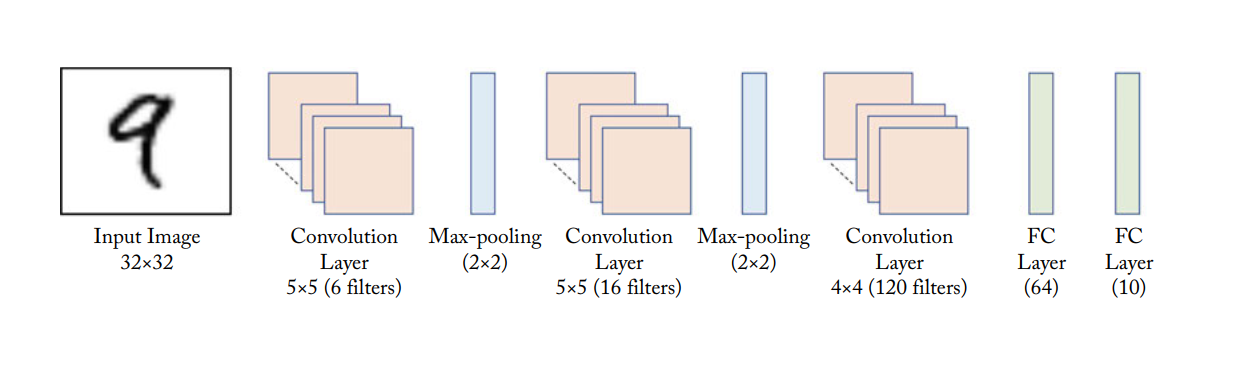
\includegraphics[width=1\textwidth]{./img/lenet}
\end{figure}


\paragraph{AlexNet} Em 2012, a vencedora do ILSVRC foi a arquitetura proposta por Alex Krizhevsky, conhecida como AlexNet, ilustrada na Figura \ref{img:alexnet}. A AlexNet é mais profunda e uma versão muito mais ampla da arquitetura LeNet \cite{ref:satapathy}. A principal diferença entre a AlexNet e as CNNs predecessoras é a sua maior profundidade, que lida muito bem com sua grande quantidade de parâmetros, além da utilização de artifícios como \textit{dropout} e \textit{data augmentation}. As cinco primeiras camadas da arquitetura AlexNet são camadas de convolução e \textit{pooling} alternadas de forma similar à LeNet, porém, seguem-se mais duas camadas uma convolucional e uma de\textit{pooling}. As três últimas camadas são FCL, mas além destas existem camadas \textit{dropout} que ajudam à reduzir \textit{overfiting} \cite{ref:khan}. \todo{Acho que a citação para alexnet está errada.}

\begin{figure}[!ht]
	\centering
	\caption{Arquitetura da AlexNet. Fonte: \cite{ref:khan}.}
	\label{img:alexnet}
	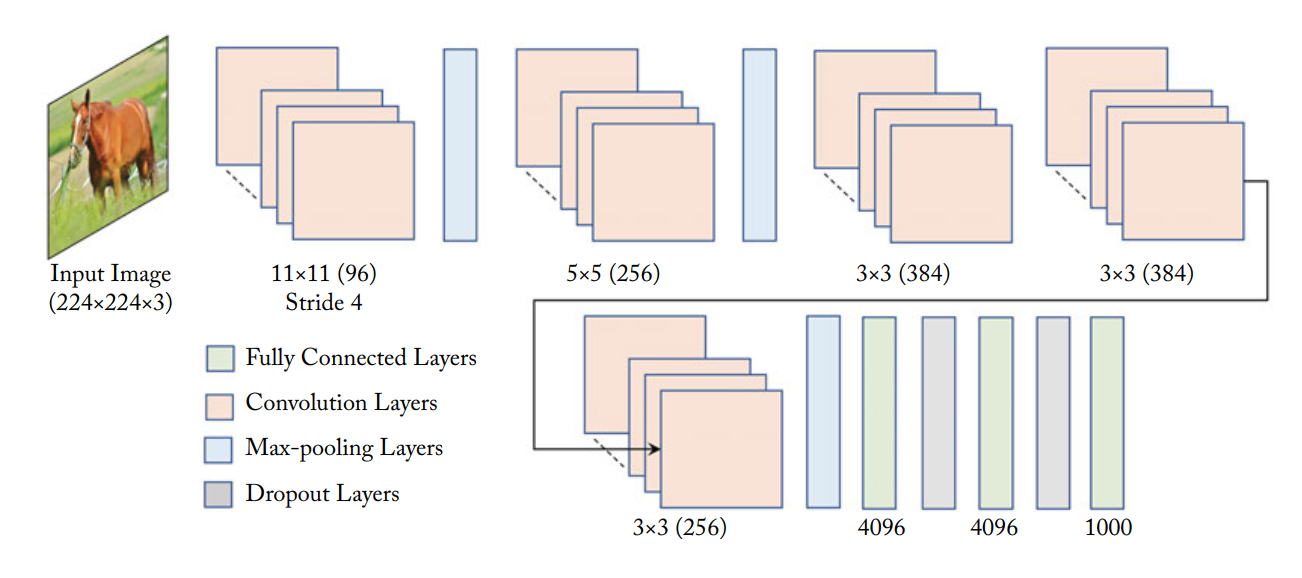
\includegraphics[width=1\textwidth]{./img/alexnet}
\end{figure}

\paragraph{VGGNet} A arquitetura VGGNet é uma das arquiteturas mais populares desde sua criação em 2014, apesar de não ter sido a vencedora do ILSVRC realizado no respectivo ano. A razão de sua popularidade se dá especialmente em virtude do uso de pequenos filtros de convolução, diminuindo o número de parâmetros ajustáveis e, por conseguinte, aumentando a eficiência do treinamento. A arquitetura VGGNet usa estritamente fitros de convolução de dimensão $3 \times 3$ combinados com camadas de \textit{pooling} para extração de características e um conjunto de três FCLs. Além das camadas de convolução, \textit{pooling} e das camadas conectadas, esta arquitetura também possui as camadas \textit{dropout} como pode ser observado na Figura \ref{img:vggnet} \cite{ref:khan}.

\begin{figure}[!ht]
	\centering
	\caption{Arquitetura VGGNet. Fonte: \cite{ref:khan}.}
	\label{img:vggnet}
	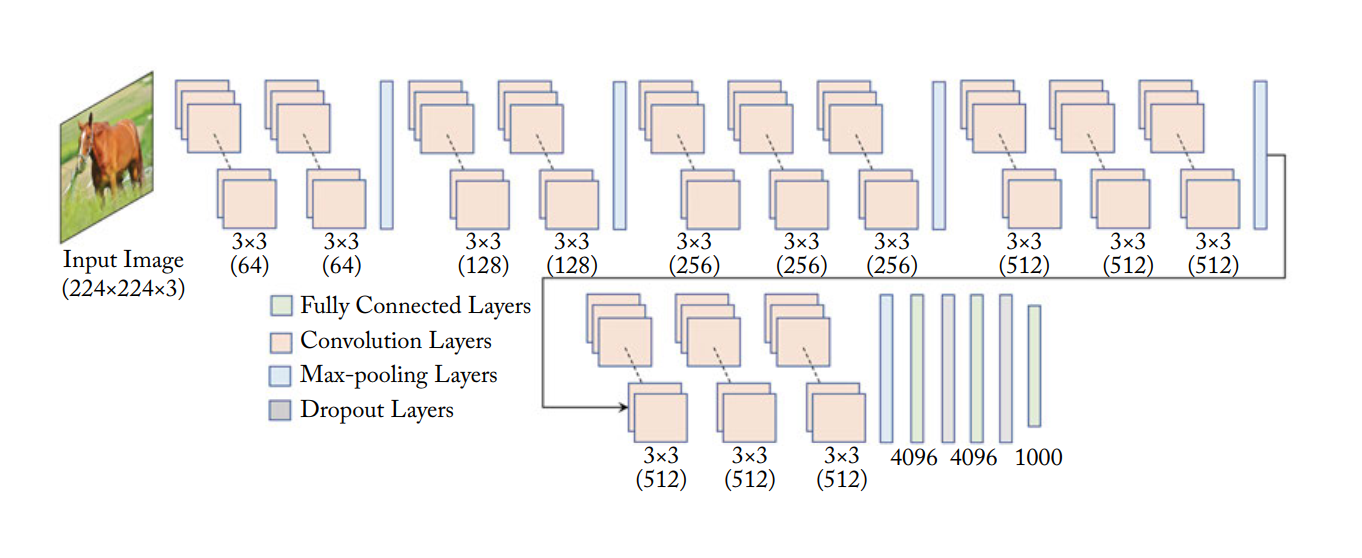
\includegraphics[width=1\textwidth]{./img/vggnet}

\end{figure}

\paragraph{GoogLeNet} Desenvolvida pela empresa Google e vencedora do ILSVRC 2014, a arquitetura GoogLeNet possui $22$ camadas baseadas em um módulo elementar chamado \emph{Inception Module}. O processamento desses módulos ocorre de forma paralela, diferentemente do processamento sequencial das arquiteturas discutidas anteriormente. A ideia central da arquitetura GoogLeNet é paralelizar os módulos e combinar as características da saída sem se preocupar com as funções individuais de cada camada. No entanto, essa abordagem resulta em um mapa de características com muitos elementos, mas para contornar este problema, após a execução do primeiro módulo, a rede realiza uma redução de dimensionalidade utilizando uma FCL antes de continuar o processo de treinamento \cite{ref:khan}. A representação da arquitetura GoogLeNet encontra-se na Figura \ref{img:googlenet}.

\begin{figure}[!ht]
	\centering
	\caption{Arquitetura GoogLeNet. Fonte: \cite{ref:khan}.}
	\label{img:googlenet}
	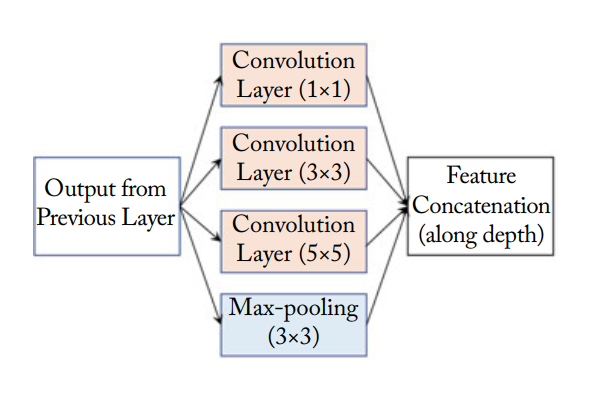
\includegraphics[width=0.6\textwidth]{./img/googlenet}

\end{figure}


\subsection{\textit{Transfer Learning}} \label{subsec:transfer}
\emph{Transfer Learning} (TL), ou Transferência de Conhecimento, é uma poderosa técnica de DL a qual possui diversas aplicações em diferentes domínios \cite{ref:gulli}. Ao invés de estruturar uma arquitetura de uma CNN e treiná-la por completo, esta técnica permite reutilizar uma rede pré-treinada e adaptá-la a um novo conjunto de dados \cite{ref:sewak}. Modelos que foram pré-treinados utilizando um vasto e genérico conjunto de dados conseguem capturar características universais, como por exemplo curvas e arestas, em suas primeiras camadas \cite{ref:zaccone}.

As técnicas de TL podem ser utilizadas de diferentes maneiras, baseando-se nas arquiteturas das CNNs. Existem alguns modelos disponíveis para aplicações que foram pré-treinados utilizando as principais arquiteturas canônicas de CNN e aprenderam as características de grandes conjuntos de dados bastante conhecidos, como o ImageNet e o Places205 \cite{ref:image-net,ref:places205}. Para diferentes tarefas, esses modelos podem ser alterados modificando a camada de saída e fazendo um retreinamento nas últimas camadas das redes para se obter o aprendizado desejado \cite{ref:khan}. 
